\section{Implementation}

\subsection{Crossfire Firefox Extension}
The first implementation of the Crossfire protocol is an extension implements
the protocol as an extension to Firefox and Firebug. The extension is
implemented entirely in JavaScript, using a modular design to allow us to share
code between client and server implementations, as well as cross-browser
implementations. This extension implements a flexible transport layer, allowing
the extension to operate as either a Crossfire client or server. This will also
enable both client and server to be implemented on top of other transport
layers, such as Web Sockets or HTTP.

The extension can be started in client or server mode either from the Firefox
user interface, or via command-line switches to Firefox. This latter mode of
operation allows external tools to launch Firefox and start the Crossfire server
listening on a known port so that the external tool may automatically connect
back to it. Figure \ref{fig:crossfire-arch}

\subsection{Crossfire Tools API}
The Crossfire extension also implements an API, called the ``Crossfire Tools API''
which enables extensibility of the Crossfire system and protocol. Firebug
features such as the Console, Inspector, and Net Panel, are implemented as tools
using the API, allowing them to be enabled/disabled independently.

\begin{figure}[htp]
  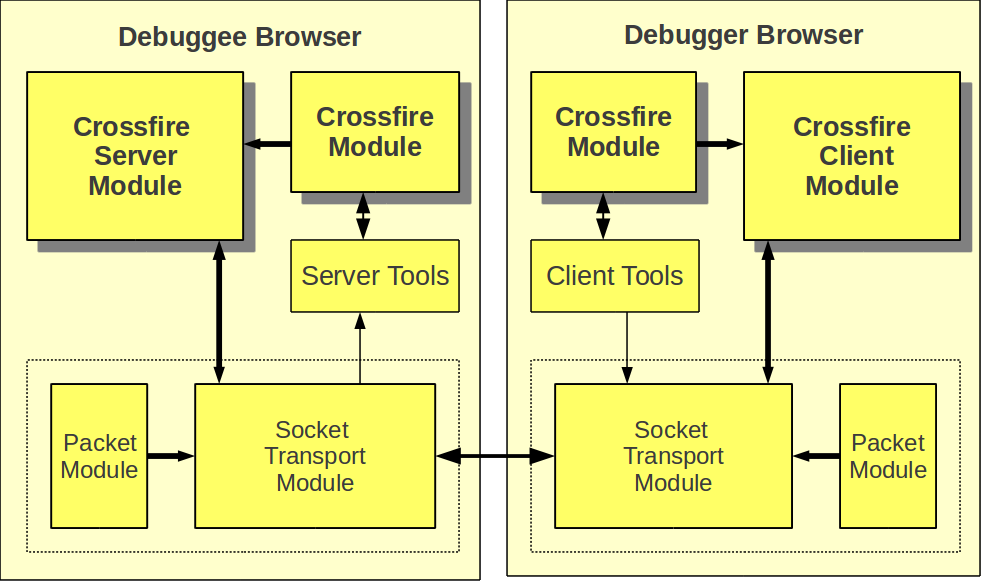
\includegraphics  [width = 86 mm] {figures/crossfire-arch4.png}
  \caption{Crossfire Firefox Extension Architecture}
 \label{fig:crossfire-arch}
\end{figure}

\subsection{Modules}

\subsection {Browser Tools Interface}